%%%%%%%%%%%%%%%%%%%%%%%%%%%%%%%%%%%%%%%%%%%%%%%
%
% Template per Elaborato di Laurea
% DISI - Dipartimento di Ingegneria e Scienza dell’Informazione
%
% update 2015-09-10
%
% Per la generazione corretta del 
% pdflatex nome_file.tex
% bibtex nome_file.aux
% pdflatex nome_file.tex
% pdflatex nome_file.tex
%
%%%%%%%%%%%%%%%%%%%%%%%%%%%%%%%%%%%%%%%%%%%%%%%

% formato FRONTE RETRO
\documentclass[epsfig,a4paper,11pt,titlepage,twoside,openany]{book}
\usepackage{epsfig}
\usepackage{plain}
\usepackage[many]{tcolorbox}
\usepackage{setspace}
\usepackage{amssymb}
\usepackage{graphicx}
\graphicspath{ {../images/} }
\usepackage[paperheight=29.7cm,paperwidth=21cm,outer=1.5cm,inner=2.5cm,top=2cm,bottom=2cm]{geometry} % per definizione layout
\usepackage{titlesec} % per formato custom dei titoli dei capitoli

\singlespacing

\usepackage[english]{babel}

\begin{document}

  % nessuna numerazione
  \pagenumbering{gobble} 
  \pagestyle{plain}

\thispagestyle{empty}

\begin{center}
  \begin{figure}[h!]
    \centerline{
\psfig{file=logo_unitn_black_center.eps,width=0.6\textwidth}}
  \end{figure}

  \vspace{2 cm} 

  \LARGE{Dipartimento di Ingegneria e Scienza dell’Informazione\\}

  \vspace{1 cm} 
  \Large{Corso di Laurea in\\
    Informatica
  }

  \vspace{2 cm} 
  \Large\textsc{Elaborato finale\\} 
  \vspace{1 cm} 
  \Huge\textsc{Understanding and classifying medical symptoms \\within a chief complaint\\}

  \vspace{2 cm} 
  \begin{tabular*}{\textwidth}{ c @{\extracolsep{\fill}} c }
  \Large{Supervisore} & \Large{Laureando}\\
  \Large{Fabio Casati}& \Large{Nicola Sartorato}\\
  \end{tabular*}

  \vspace{2 cm} 

  \Large{Anno accademico 2018/2019}
  
\end{center}



  \clearpage
 
  \thispagestyle{empty}

\begin{center}
  {\bf \Huge Acknowledgments}
\end{center}

\vspace{4cm}


\emph{\\
  My gratitude goes to...\\
  My heartfelt thanks to...\\
  Thanks to professor Casati\\
  Thanks to my family\\
  Thanks to Francesco\\
}

  \clearpage
  \pagestyle{plain} % nessuna intestazione e pie pagina con numero al centro

  % inizio numerazione pagine in numeri arabi
  \mainmatter

    % indice
    \tableofcontents
    \clearpage    
          
    % gruppo per definizone di successione capitoli senza interruzione di pagina
    \begingroup
      % nessuna interruzione di pagina tra capitoli
      % ridefinizione dei comandi di clear page
      \renewcommand{\cleardoublepage}{} 
      \renewcommand{\clearpage}{} 
      % redefinizione del formato del titolo del capitolo
      % da formato
      %   Capitolo X
      %   Titolo capitolo
      % a formato
      %   X   Titolo capitolo
      
      \titleformat{\chapter}
        {\normalfont\Huge\bfseries}{\thechapter}{1em}{}
        
      \titlespacing*{\chapter}{0pt}{0.59in}{0.02in}
      \titlespacing*{\section}{0pt}{0.20in}{0.02in}
      \titlespacing*{\subsection}{0pt}{0.10in}{0.02in}
      
      % sommario
      \chapter*{Abstract} % senza numerazione
\label{abstract}

\addcontentsline{toc}{chapter}{Abstract} % da aggiungere comunque all'indice

%%%%%%%%%%%%%%%%%%%%%%%%%%%%%%%%%%%%%%%%%%%%%%%%%%%%%%%%%%%%%%%%%%%%%%%%%%%%%%%%
%% Sommario è un breve riassunto del lavoro svolto dove si descrive l'obiettivo, l'oggetto della tesi, le 
%% metodologie e le tecniche usate, i dati elaborati e la spiegazione delle conclusioni alle quali siete arrivati.  
%%
%% Il sommario dell’elaborato consiste al massimo di 3 pagine e deve contenere le seguenti informazioni:
%%  - contesto e motivazioni 
%%  - breve riassunto del problema affrontato
%%  - tecniche utilizzate e/o sviluppate
%%  - risultati raggiunti, sottolineando il contributo personale del laureando
%%
%% Summary:
%%
%%  - briefly and abstractly explain the problem and what my code does (example from dataset, image)
%%    - 2 objectives:
%%      - identify for each symptom a part of sentence related to it (this are intelligible tokens and then can be printed in the final report)
%%      - mapping these parts of sentences in a specific symptom identified by a CUI
%%    - my work is part of a bigger project: an history taking chatbot (image)
%%      - what is the aim of the history taking chatbot?
%%      - why is it useful to map the symptoms towards a classification of symptoms?
%%        - briefly tell what is MEDCIN and UMLS classification
%%
%%  - why history taking? => document john
%%    - why is it necessary? What does a physician lack? => document john
%%      - lack of physicians on rural areas / less populated areas (Philippines example)
%%      
%%  - abstract but more detailed paragraph about code and techniques
%%    - used techniques
%%    - developed techniques
%%    
%%  - results
%%    - QA system results
%%    - mapping towards a classification results
%%%%%%%%%%%%%%%%%%%%%%%%%%%%%%%%%%%%%%%%%%%%%%%%%%%%%%%%%%%%%%%%%%%%%%%%%%%%%%%%
  
      
      %%%%%%%%%%%%%%%%%%%%%%%%%%%%%%%%
      % lista dei capitoli
      %
      % \input oppure \include
      %
      
      \chapter{Overview}
\label{cha:intro}

\section{The major problem of physicians: time}
\label{sec:problem_doctors}
Physicians all over the world visit patients under time limitations. In addition, in underdeveloped countries there is not always a suitable doctor-population ratio (1:1000 is the optimal ratio according to the World Health Organization)\cite{johndocument}: thus, doctors in those places may be overloaded with work. Hence, the main problem of physicians is time. This obviously affects the way in which doctors examine patients, especially the anamnesis elicitation, which is the most time-consuming task during medical examinations.

\subsection{The anamnesis elicitation: a crucial but time-consuming task}

The anamnesis of a patient is the information gained by a physician by asking specific questions whose answers may be useful in formulating a diagnosis\cite{historytakingwiki}. This task, often called in medical jargon “history taking”, requires a long procedure because the physician does not have only to interview the patient and gather information about the history of their problem, but even write down a brief summary of the conversation in the patient’s record. This necessary bureaucracy is demanding and risks becoming all-embracing. For example, a research group monitoring 57 physicians in the United States observed that during the clinic day, physicians were spending 49.2\% of their clinical time on health records and desk work and only 27\% of their time with patients \cite{sinsky}. However, this task is fundamental: according to research, medical history provides in the 82.5\% of patients enough information to make an initial diagnosis of a disease \cite{hampton1975}.

The traditional way of interviewing the patient is not only long and demanding, but even sometimes incomplete. For instance, 134 primary care physicians observed that, during the study, only 59\% of essential history items were collected during history taking. Physicians were able to obtain relevant information about presenting symptoms and medications, but they often missed important information about related symptoms and medical history. This because a physician needs to remember a large number of questions and symptoms to have a complete and accurate history. Human memory is fallible and forgetting to ask some relevant questions during an interview might have a significant implication in patient management.\cite{johndocument}

\subsection{An alternative to the traditional anamnesis elicitation}

Therefore, it is for the aforementioned reasons that a new approach to anamnesis should be tried. Digitize this task is a possible solution which is time-saving for physicians and, at the same time, could provide a better history taking outcome. The ideal interaction model between this history taking program and the patient is a chat conversation. Basically, the patient, chatting, interacts with this conversational software, which has to understand and classify the presenting symptoms and, later, elicit symptoms and information useful for the diagnosis that the patient may have forgotten. A first obstacle towards an effective history taking chatbot is identifying and classifying symptoms within a patient’s answer. This work is focused on it.

\section{What does identifying and classifying symptoms mean?}

This section is dedicated to present a high level view of the work and the two main abstract components of the code: the \textit{Symptom Identifier} and the \textit{Symptom Classifier}. 

\label{sec:identifying_classifying}
\subsection{Identifying symptoms}

Identifying symptoms within a patient's sentence means finding, inside the text of the sentence, every group of adjacent words that carry together a coherent symptom concept.

\begin{figure}[h]
\centering
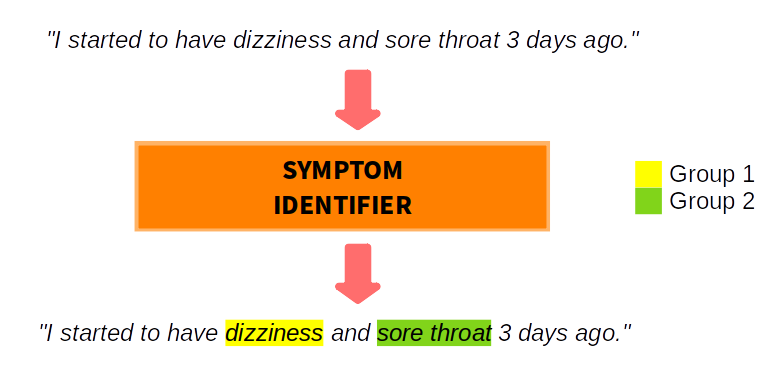
\includegraphics[width=12cm]{symptom_identifier}
\caption{The \textit{Symptom Identifier} seen abstractly.}
\medskip
\end{figure}
\newpage
These groups of words will then be mapped into precise symptoms contained in a symptom classification: they are named \textit{tokens for predictions} (TFPs for short).

\subsection{Classifying symptoms}
\label{sec:cla_symp}

Thus, the objective of the Symptom Classifier is to map correctly the previous \textit{tokens for predictions} into a list of specific symptoms. Each symptom inside the classification has an unique identifier called CUI (Concept Unique Identifier). The first character of a CUI is a \texttt{C} followed by seven digits.

\begin{figure}[h]
\centering
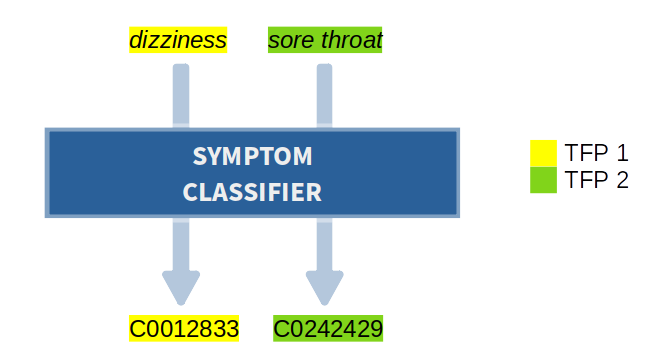
\includegraphics[width=10cm]{symptom_classifier}
\caption{The \textit{Symptom Classifier} seen abstractly.}
\medskip
\end{figure}

\subsubsection{The MEDCIN symptom classification}
MEDCIN is a medical terminology system developed by Medicomp Systems Inc. \cite{medcin}. It contains more than $300\,000$ clinical data elements encompassing symptoms, physical examinations, tests, diagnoses and therapies. What makes MEDCIN particularly fit for the purpose of this work is its nature of being a \textit{point of care} terminology system. This means that MEDCIN is intended to help clinicians in documenting clinical information while interacting with patients. Therefore, MEDCIN includes all the symptom concepts that a physician may need when summarizing a patient's problem. In addition, another positive aspect stands in its hierarchical organization: the symptoms are structured in a tree, and each child of a node is in a \textit{is-a} relationship with its father.

Although MEDCIN is copyrighted, it is inside the list of supported UMLS terminology systems. The Unified Medical Language System (UMLS) is a compendium of many controlled medical vocabularies and it is maintained by the US National Library of Medicine \cite{umls}. Academic users may access the UMLS free of charge for research purposes.

Encompassing MEDCIN, UMLS provides a mapping structure between it and any other terminology system supported by UMLS. This is positive because CUIs are codes which are transversal to all the vocabularies inside the UMLS.

\subsubsection{But why is  classifying symptoms necessary?}
Find an appropriate mapping for a \textit{token for prediction} is not a trivial task, mainly because reality is not easily classifiable; natural language in particular. However, mapping symptoms to a classification is useful especially for improving the quality of the chatbot. This because the long-term objective is not to understand the presenting symptoms (physicians, and, generally, every human, are very good at it) but ask clever questions to the patient in order to extract missing symptoms and, in general, useful information for the diagnosis. This could be done asking questions about related symptoms or reviewing the body systems (Review of Systems (ROS) is normal practice in history taking). For these reasons, a mapping to a standard symptom classification is essential.

\section{Brief description of methods}
\label{sec:brief_methods}

This section will briefly outline the methods that has been developed and the technologies that has been used. Then, chapter \ref{cha:methods} will deepen more into the details of the components listed below.

\subsection*{Symptom identifier}
The abstract component \textit{Symptom Identifier} is made up of three sub-components:
\begin{itemize}
  \item a \textit{Body Part Finder}. Its aim is to identify words that are common body parts inside the sentence. The purpose is to find them and later inform the next component about the body parts that appeared within the sentence;
  \item a \textit{Question Answering (QA) system}. The objective of this component is, given a set of questions, aswering them highlighting the parts of the sentence which respond to each question. This task is called \textit{Maching Reading Comprehension} and can be done with these two supported models:
    \begin{enumerate}
      \item \textit{BERT}, that stands for \textit{Bidirectional Encoder Representations from Transformers} \cite{bert}, finetuned on \textit{SQuAD} (a Reading Comprehension dataset developed by Stanford University) \cite{squad};
      \item \textit{R-NET}, an end-to-end neural networks model for Reading Comprehension developed by Microsoft  \cite{rnet};
    \end{enumerate}
  \item an \textit{Answer Interpreter}. In this stage the answers of the previous component (the \textit{QA system}) become \textit{tokens for predictions}: this prepares them for the vectorization.
\end{itemize}

\subsection*{Symptom classifier}
The abstract component \textit{Symptom Classifier} is made up of two sub-components:
\begin{itemize}
  \item a \textit{Vectorifier}. The purpose of this component is encoding a given sentence into an embedding which can be of two types:
  \begin{enumerate}
    \item \textit{GloVe} embedding \cite{glove};
    \item \textit{BERT} embedding;
  \end{enumerate}
  \item a \textit{Symptom Tree Mapper}. The aim of this component is returning, given the embedding of a \textit{token for prediction}, the CUI of the most similar symptom. Similarity is a suitable measure because both the \textit{tokens for predictions} and each symptom name can be vectorized; thus, for both of them, an internal representation is available.
\end{itemize}

\subsection*{Dataset}
\label{datasetintro}
Up to now, there are not any suitable datasets for this project; therefore, for the purpose of this work, it proved necessary scraping and tagging $336$ sentences extracted from posts of a medical forum \footnote{\url{https://www.doctorslounge.com/forums/}} \cite{doctorslounge}. In section \ref{sec:dataset} is described the process that was followed in order to create this dataset.

\section{Brief description of results}
\label{sec:brief_results}
As shown in chapter \ref{cha:results}, BERT is better than R-NET in identifying symptoms. As a matter of fact, using BERT, the percentage of correct tokens is $84.8 \%$, while, using R-NET it is of $70.4 \%$ ($+ 14.4 \%$ of improvement). BERT for QA outperforms R-NET even in other indices presented in section \ref{sec:eval_symptom_identifier}.

In section \ref{sec:evalsymptomclassifier}, any option of the Symptom Classifier is analyzed one by one: this means testing the model with different embedding types, if using or not the Body Part Finder and other options such as \textit{pruning}, filtering ``useless words'' and the minimum similarity threshold that will be treated in the corresponding section.

      
      \chapter{Methods}
\label{cha:methods}
In this chapter I will describe in detail the methods used in order to achieve the results described in the next chapter. In the following sections I will analyze the abstract components illustrated in the Introduction.

\section{The \textit{Body Part Finder}}
\label{sec:body_part_finder}
\subsection{The body part list}
The objective of this component is to identify body parts words within the patient's sentence. For doing so, it is obviously necessary to have a list of body parts. In addition, each body part can be expressed by the patient using a large variety of terms (its synonyms). Hence, with the addition of an abstraction layer, the list of body parts becomes a list of body parts concepts; and each body part concept is associated with a list of its synonyms. Another problem to face is that the language of this body parts classification should be at “patient level”: therefore it has to be informal and not strictly medical.

Unfortunately, I did not find any body part classification with these features. Therefore, the only chance for me was to produce my own classification, starting my work from the numerous informal body part lists that I found searching the Web. I based my classification mainly on the Wikipedia's list of body parts[], which I completed with other missing body parts found in other lists. I understand the licit perplexities that this approach may arise. However, in my opinion, what really matters is that, even with this amateur list of body parts, the results make my proof of concept creditable, as we will see in the next chapter. The classification is composed of [130] body parts saved in a csv file.

\subsection{Finding a body part in a sentence}
Finding a body part in a sentence is quite easy if you have an exhaustive list of body parts and the respective synonyms. The code does nothing more than a string matching between each word in the sentence and each synonym present inside the classification. This approach is simple but not perfect: for example, the word “back” is both a preposition and a body part. Therefore, looking only at words means forgetting the context: this may introduce misunderstandings and lower the quality of the results.
%% TODO scrivo che c'e' da migliorare

\section{Question-Answering system}
\label{sec:qa_system}
The outcome of the \textit{Body Part Finder} is then passed to the \textit{QA system}, whose basic aim is to give an answer to questions like “What are the symptoms in the sentence?” or “What is the problem with the neck?”. If the reader has never heard of Machine Reading Comprehension, this may seem magic. However, fortunately, as we will see in this section, it is not.

\subsection{Types of questions}
The questions asked to the specified model over each sentence are of two types:
\begin{enumerate}
  \item generic question about the symptoms in the sentence (“What are the symptoms?”)
  \item specific question about the problem of a found body part in the sentence (“What is the problem with the [body part]?”)
\end{enumerate}

The question over the symptoms is intentionally generic because its aim is to catch the majority of the symptoms within the sentence. Thus, as we will see in the next section, the answer to this question should be interpreted.

At the same time, the question over a body part is deliberately specific. The logic behind this question is that if a patient refers to a body part during the interview, perhaps it is the subject of a problem.

Here is a figure in order to understand the whole component:

%% IMAGE ABOUT QA SYSTEM
\begin{figure}[h]
\centering
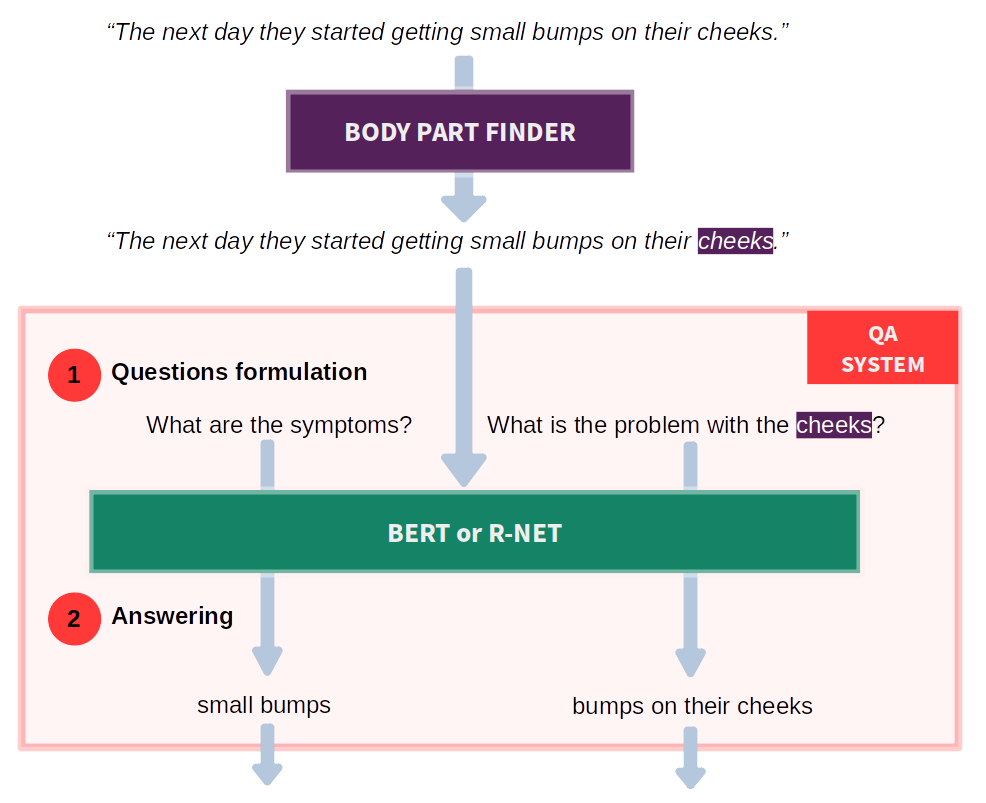
\includegraphics[width=14cm]{qa_sys}
\caption{The \textit{QA system} illustated.}
\medskip
\end{figure}

If we look at the answers of this figure, we can understand two problems: the model can sometimes provide an useful answer but too generic (this is the case of ``small bumps'') and might provide redundant answers, increasing unnecessarily the number of predictions.

%% domenica
\subsection{BERT}
Even if I did not personally fine-tuned BERT on SQuAD (I used DeepPavlov's pretrained BERT-SQuAD \cite{deeppavlov}), in this subsection I will briefly outline the characteristics that made BERT a revolutionary model.

BERT, which stands for Bidirectional Encoder Representations from Transformers, is a new language representation model. Even if BERT was presented to the research world in May 2019, it has yet obtained new state-of-the-art results on eleven natural language processing tasks. For instance, a finetuned BERT push SQuAD v1.1 question answering F1 Test to 93.2 (1.5 points of absolute improvement) and SQuAD v2.0 F1 Test to 83.1 (5.1 points of absolute improvement) \cite{bert}.

The training framework proposed by Devlin et al., the authors of BERT, is composed of two steps: \textit{pre-training} and \textit{fine-tuning}. During pre-training BERT is trained over different pre-training tasks. The fine-tuning is only over a single downstream task, in our case, the SQuAD task.

% https://arxiv.org/pdf/1706.03762.pdf
BERT’s  model  architecture is a multi-layer bidirectional Transformer encoder. These last components, that are the building blocks of BERT, are implemented as described in the paper \textit{Attention Is All You Need} by Vaswani et al. \cite{attentionisallyouneed}.

Considering BERT Base, the size taken in consideration for this project (the choice was between Base and Large), the hidden layers (i.e. Transformers encoders) are 12, the hidden size is 768 and the number of self-attention heads is 12.

\begin{figure}[t]
\centering
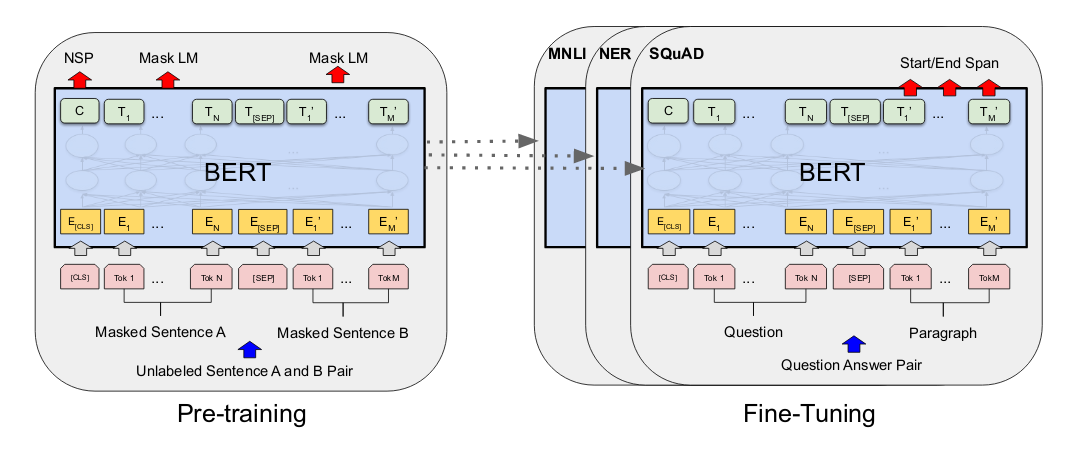
\includegraphics[width=18cm]{bert-for-squad-original-paper}
\caption{Overall pre-training and fine-tuning procedures for BERT. The pre-training procedure provides a basis for the numerous possible downstream tasks. \texttt{[CLS]}, which stands for ``classification'', is a special symbol added in front of every input example, and \texttt{[SEP]} is a special separator token. For further information about the input representation, please read the paper linked in the references. This image is extracted by that paper (\cite{bert}).}
\medskip
\label{fig:bertsquad}
\end{figure}

\subsubsection{Pre-training BERT}
Briefly, pre-training BERT means training it on two tasks:
\begin{itemize}
  \item \textit{Masked Language Model} (MLM), often called \textit{Cloze task}. A bidirectional model like BERT is undoubtedly more powerful than a left-context model like the OpenAI GPT Transformer. But this type of model is even more difficult to train because a bidirectional conditional language model cannot be trained left-to-right or right-to-left, since this would allow each word to indirectly “see itself” during training. Thus, in order to train a bidirectional representation, the researchers simply mask some percentage of the input tokens at random (15\% in their experiments), and then predict those masked tokens. Masking a tokens means substitute a real token with a placeholder token \texttt{[MASK]}. 
  \item \textit{Next Sentence Prediction} (NSP). This task is beneficial to many important downstream tasks like Question Answering and Natural Language Inference that are based on understanding the relation between two sentences, skill that is not captured by the previous task. Basically, this task is a binary \textit{next sentence prediction}: when choosing the sentences \texttt{A} and \texttt{B} for the training, in the 50\% of the cases \texttt{B} is an actual next sentence of \texttt{A} (and it is labeled as \texttt{IsNext}) while in the other cases the choice of \texttt{B} is random between the sentences (labeled as \texttt{NotNext}).
\end{itemize}

% https://arxiv.org/pdf/1606.05250.pdf
\subsubsection{A dataset for Reading Comprehension: SQuAD}
In the fine-tuning stage BERT is trained on SQuAD, a dataset for Reading Comprehension developed by Stanford University \cite{squad}. It consists in a collection of $100\,000$ question-answer pairs over different Wikipedia passages. There are two versions of SQuAD: the first version (\texttt{v1.1}) contains only questions over a passage that have an answer, while the second version (\texttt{v2.0}) have some questions without answer. Obviously, doing better on SQuAD 2.0 is more difficult, because it requires a minimum level of reasoning.

\subsubsection{Fine-tuning BERT on SQuAD1.1}
As illustrated in Figure \ref{fig:bertsquad}, during fine-tuning passage and question are both passed to BERT (separated by the \texttt{[SEP]} tag). This phase introduces two trainable vectors: $S$ (for the start of the answer) and $E$ (for the end of the answer) both of dimension $\mathbb{R}^\mathbb{H}$ ($\mathbb{H}$ is the hidden size, $768$ for BERT Base). 

The probability of a token $i$ of being the start of the answer is $P_{i} = \frac{\mathrm{e}^{S \cdot T_{i}}}{\sum_{j} \mathrm{e}^{S \cdot T_{j}}}$, where $T$ here represents the last layer of BERT. The analogous formula is used for the end of the answer. The score of a candidate span that goes from token $i$ to token $j$ is defined as $score_{i, j} = S \cdot T_{i} + E \cdot T_{j}$. The maximum score where $j \geq i$ is used as prediction. Finally, the training objective is defined as the sum of the two log-likelihoods \eqref{eqn:loglikelihood} of the correct start and end positions.

\begin{equation}
\label{eqn:loglikelihood}
loglikelihood(S) = \sum_{i} y_{i} \mathrm{ln} (P(y_{i} | S)) + (1 - y_{i}) \mathrm{ln} (1 - P(y_{i} | S))
\end{equation}


\subsection{R-NET}
This section will briefly outline R-NET, the other model used for Reading Comprehension. R-NET is trained on SQuAD, dataset described in section \ref{squad}.

R-NET is an end-to-end neural networks model for reading comprehension \cite{rnet}. It performs this task similarly to the way a human does: reading the passage (i.e. the patient's sentence) multiple times. Basically, R-NET tries to improve the passage representation step after step, which are in total three:
\begin{enumerate}
  \item \textit{Question and Passage GRU Layer}. In this layer tokens are converted in GloVe embeddings, and for out-of-vocabulary tokens a character embedding is computed. These vectors are not contextual: for this reason these embeddings are then fed to a BiRNN (composed by Gated Recurrent Units \cite{gru}) in order to ameliorate these representations.
  \item \textit{Question and Passage Matching Layer}. The aim of this layer is to encode the question terms into the passage embeddings of the previous layer. In other words, this permits to the network, given a token in the passage, to focus only on the relevant tokens in the question and tune the passage embeddings to be more similar to the relevant question vectors. This is done using \textit{Attention}.
  
In order to explain this concept, the example taken from \cite{understandingrnet} is reported.

Assuming we are at the highlighted word in the passage:

\begin{displayquote}
She had a talent for \textit{making} home craft tools, mechanical appliances, and the ability to memorize Serbian epic poems.
\end{displayquote}

Given the highlighted token \textit{making}, Attention over the question tokens will highlight the word in italic:

\begin{displayquote}
What were Tesla's mother's special \textit{abilities}?
\end{displayquote}

In this case, \textit{making} embedding is adjusted in order to get it closer to \textit{abilities} embedding. With this procedure, R-NET encodes the question in the passage.

  \item \textit{Passage Self-Matching Layer}. Consider the following passage:
  
  \begin{displayquote}
  Tesla’s mother, Đuka Tesla (née Mandić), whose father was also an Orthodox priest, had a talent for making home craft tools, mechanical appliances, and the \textit{ability} to memorize Serbian epic poems. Đuka had never received a formal education. Nikola credited his eidetic memory and creative \textit{abilities} to his mother’s genetics and influence.
  \end{displayquote}
  
  It is clear that the term \textit{ability} refers to the mother of Tesla, while \textit{abilities} refers to Nikola Tesla. The objective of this step is to capture the difference between terms like those, that, without context, are identical.
  
  Another difficulty resides in \textit{long-term dependencies}: \textit{ability}, for example, is far away from the subject to which the term is referred (Tesla's mother). However, GRU \cite{gru} were developed for addressing the problem of the \textit{vanishing gradients}, which is the reason why vanilla RNNs have troubles with long-term dependencies.
  
  To resolve the former problem, R-NET introduces \textit{Self-Matched Attention}. While with simple Attention a passage term is used to weight a set of vectors (the question terms), with Self-Matched Attention R-NET uses the current passage term to weigh tokens from the passage itself. This helps to make clearer the meaning between ambiguous terms.
\end{enumerate}

Having read and analyzed for three times the passage in the light of the question, the last layer is aimed to output the start and the end of the answer within the passage.

\begin{figure}[t]
% https://slideplayer.com/slide/12351679/
\centering
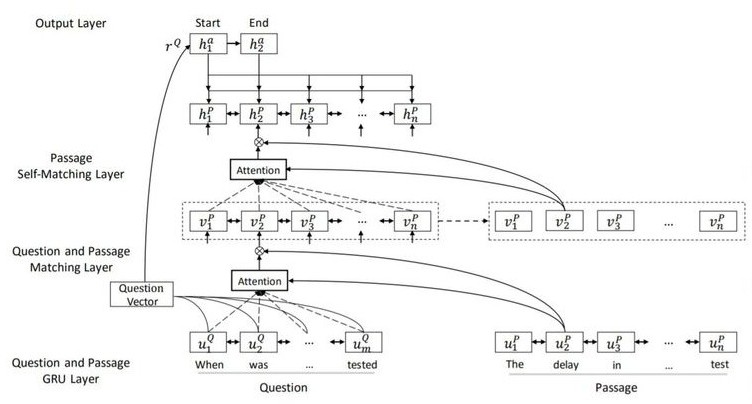
\includegraphics[width=15cm]{rnet}
\caption{A simplified overview of R-NET \cite{imagernetoverview}}
\medskip
\end{figure}



%% lunedi
\section{Answer Interpreter}
\label{sec:answer_interpreter}
This component receives the answers of the Question Answering system, interprets them and outputs the \textit{tokens for predictions}.

\subsection{Stemming}
\label{sec:stemming}
Before the interpretation, the answers are stemmed using the \textit{Snowball Stemmer} present in NLTK with a slight modification \cite{snowballstemmer, nltk}. This because it is true that the stemming reduces the variability of text, mapping inflected or derived words into their root form (the stem); but it is also true that a stem does not need to be identical to the morphological word root. This is a problem because a stemmer might output out-of-vocabulary words, which cannot be vectorified. Thus, the solution stands in accepting the stemmed word only if it is inside the vocabulary (the list of the first $100\,000$ terms in GloVe pre-trained embeddings). This stemmer is also used in the calculation of the representative embeddings of symptoms.

\subsection{Filtering ``useless words''}
The stemmed answers are then passed to a function that filters ``useless words''. Basically, it keeps only words that are tagged as a \textit{part of speech} that is inside the following list: noun, adjective, coordinating conjunction, punctuation, verb and auxiliar. For this purpose the Stanford POS Tagger, which is inside Stanford NLP library \cite{stanfordnlp}, was used. Thus, the basic idea is to simplify the answer deleting words like adverbs and pronouns that do not contribute to the meaning of the symptoms.

\subsection{Answer interpretation}
The two different types of answers are processed in a different way:
\begin{itemize}
  \item the general answer about symptoms is one for each passage. Usually, this answer contains more symptoms separated by a coordinating conjunction: mainly, the comma and ``and''. For this reason, the Answer Interpreter splits the answer on these terms and originates one or more \textit{tokens for predictions}.
  \item the specific answers about a body part are as many as the number of body parts found in the passage. Given a body-part answer, the \textit{token for prediction} is formed concatenating the answer with the name of the body part.
\end{itemize}

\begin{figure}[h]
\centering
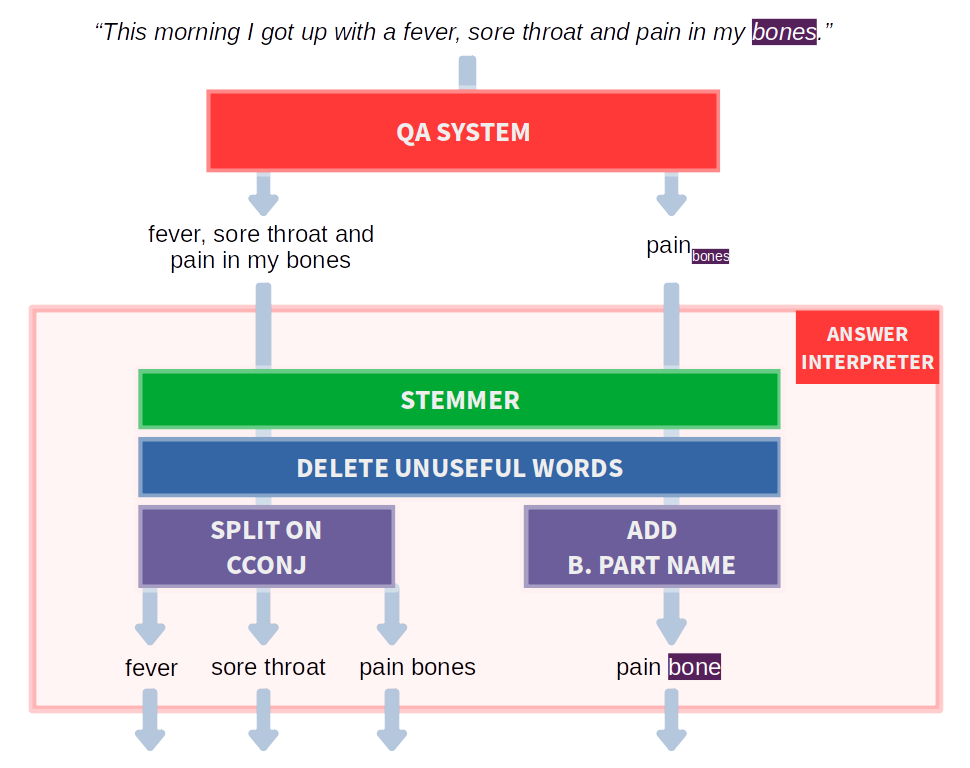
\includegraphics[width=13cm]{answer_interpreter}
\caption{The Answer Interpreter illustrated.}
\medskip
\label{fig:answer_int}
\end{figure}



\section{Vectorifier}
\label{sec:body_part_finder}
TODO

\section{Symptom Tree Mapper}
\label{sec:symptom_tree_mapper}
\subsection{Symptom Tree}
TODO, representation in anytree, from mysql following refto

\subsection{Mapping of a token for prediction to a specific symptom}
TODO


%% martedi'
\section{How to evaluate results?}
\label{sec:eval_results}
TODO


\section{How to find an internal representation of a symptom?}
Use the concept name and vectorize the sentence (with glove)
Prima fai lo stemming pero', justify it, reduce the space of mapping. possibile figura


\section{Dataset}
site I visited
"extrapolating sentences within the posts" in which there were classifiable symptoms wrt the classification
format of the sentences: xml tags, sentence tag
      
      %%%%%%%%%%%%%%%%%%%%%%%%%%%%%%%%
      
      
    \endgroup


    % bibliografia in formato bibtex
    %
    % aggiunta del capitolo nell'indice
    \addcontentsline{toc}{chapter}{Bibliografia}
    % stile con ordinamento alfabetico in funzione degli autori
    \bibliographystyle{plain}
    \bibliography{biblio}

    \titleformat{\chapter}
        {\normalfont\Huge\bfseries}{Allegato \thechapter}{1em}{}
    % sezione Allegati - opzionale
    \appendix
    %\chapter{Titolo primo allegato}

Lorem ipsum dolor sit amet, consectetur adipiscing elit. Donec sed nunc orci. Aliquam nec nisl vitae sapien pulvinar dictum quis non urna. Suspendisse at dui a erat aliquam vestibulum. Quisque ultrices pellentesque pellentesque. Pellentesque egestas quam sed blandit tempus. Sed congue nec risus posuere euismod. Maecenas ut lacus id mauris sagittis egestas a eu dui. Class aptent taciti sociosqu ad litora torquent per conubia nostra, per inceptos himenaeos. Pellentesque at ultrices tellus. Ut eu purus eget sem iaculis ultricies sed non lorem. Curabitur gravida dui eget ex vestibulum venenatis. Phasellus gravida tellus velit, non eleifend justo lobortis eget. 

\section{Titolo}
Lorem ipsum dolor sit amet, consectetur adipiscing elit. Donec sed nunc orci. Aliquam nec nisl vitae sapien pulvinar dictum quis non urna. Suspendisse at dui a erat aliquam vestibulum. Quisque ultrices pellentesque pellentesque. Pellentesque egestas quam sed blandit tempus. Sed congue nec risus posuere euismod. Maecenas ut lacus id mauris sagittis egestas a eu dui. Class aptent taciti sociosqu ad litora torquent per conubia nostra, per inceptos himenaeos. Pellentesque at ultrices tellus. Ut eu purus eget sem iaculis ultricies sed non lorem. Curabitur gravida dui eget ex vestibulum venenatis. Phasellus gravida tellus velit, non eleifend justo lobortis eget. 

\subsection{Sottotitolo}
Lorem ipsum dolor sit amet, consectetur adipiscing elit. Donec sed nunc orci. Aliquam nec nisl vitae sapien pulvinar dictum quis non urna. Suspendisse at dui a erat aliquam vestibulum. Quisque ultrices pellentesque pellentesque. Pellentesque egestas quam sed blandit tempus. Sed congue nec risus posuere euismod. Maecenas ut lacus id mauris sagittis egestas a eu dui. Class aptent taciti sociosqu ad litora torquent per conubia nostra, per inceptos himenaeos. Pellentesque at ultrices tellus. Ut eu purus eget sem iaculis ultricies sed non lorem. Curabitur gravida dui eget ex vestibulum venenatis. Phasellus gravida tellus velit, non eleifend justo lobortis eget. 


\chapter{Titolo secondo allegato}

Lorem ipsum dolor sit amet, consectetur adipiscing elit. Donec sed nunc orci. Aliquam nec nisl vitae sapien pulvinar dictum quis non urna. Suspendisse at dui a erat aliquam vestibulum. Quisque ultrices pellentesque pellentesque. Pellentesque egestas quam sed blandit tempus. Sed congue nec risus posuere euismod. Maecenas ut lacus id mauris sagittis egestas a eu dui. Class aptent taciti sociosqu ad litora torquent per conubia nostra, per inceptos himenaeos. Pellentesque at ultrices tellus. Ut eu purus eget sem iaculis ultricies sed non lorem. Curabitur gravida dui eget ex vestibulum venenatis. Phasellus gravida tellus velit, non eleifend justo lobortis eget. 

\section{Titolo}
Lorem ipsum dolor sit amet, consectetur adipiscing elit. Donec sed nunc orci. Aliquam nec nisl vitae sapien pulvinar dictum quis non urna. Suspendisse at dui a erat aliquam vestibulum. Quisque ultrices pellentesque pellentesque. Pellentesque egestas quam sed blandit tempus. Sed congue nec risus posuere euismod. Maecenas ut lacus id mauris sagittis egestas a eu dui. Class aptent taciti sociosqu ad litora torquent per conubia nostra, per inceptos himenaeos. Pellentesque at ultrices tellus. Ut eu purus eget sem iaculis ultricies sed non lorem. Curabitur gravida dui eget ex vestibulum venenatis. Phasellus gravida tellus velit, non eleifend justo lobortis eget. 

\subsection{Sottotitolo}
Lorem ipsum dolor sit amet, consectetur adipiscing elit. Donec sed nunc orci. Aliquam nec nisl vitae sapien pulvinar dictum quis non urna. Suspendisse at dui a erat aliquam vestibulum. Quisque ultrices pellentesque pellentesque. Pellentesque egestas quam sed blandit tempus. Sed congue nec risus posuere euismod. Maecenas ut lacus id mauris sagittis egestas a eu dui. Class aptent taciti sociosqu ad litora torquent per conubia nostra, per inceptos himenaeos. Pellentesque at ultrices tellus. Ut eu purus eget sem iaculis ultricies sed non lorem. Curabitur gravida dui eget ex vestibulum venenatis. Phasellus gravida tellus velit, non eleifend justo lobortis eget. 




\end{document}
